\newcommand{\wimp}{\w_{\avg{E_v}}}
\newcommand{\wsw}{\w_{B_r}}
\newcommand{\wedm}{\w_{edm}}

\newcommand{\D}{\Delta}
\DeclareDocumentCommand{\g}{s}{\gamma\IfBooleanT{#1}{_{eff}}}

\subsection{Метод BNL FS \label{sec:BNL-FS-method}}
В 2008 году коллаборацией srEDM (Storage Ring EDM),~\cite{BNL:SREDM}  занимающейся разработкой
метода измерения ЭДМ в накопительном кольце в Брукхейвенской
Национальной Лаборатории (США), был предложен метод~\cite{BNL:Deuteron2008}
измерения ЭДМ в комбинированном накопительном кольце. В рамках данного исследования, 
обозначим его как ``BNL FS'' метод. 

В BNL FS методе пучок продольно-поляризованных дейтронов инжектируется в кольцо. 
Посредством поляриметрии наблюдается его спин-прецессия в вертикальной и горизонтальной плоскостях. 
ЭДМ сигнал --- это изменение вертикальной компоненты поляризации со временем, 
выражаемое как:~\cite[стр.~8]{BNL:Deuteron2008}
\begin{equation}
  \Delta P_V = P\frac{\w_{edm}}{\W}\sin\bkt{\W t + \Theta_0},
\end{equation}
где $\W = \sqrt{\w_{edm}^2 + \w_a^2}$; $\w_a,~\w_{edm}$ частоты прецесси спина,
связанные, соответственно, с магнитным и электрическим дипольными моментами. 
Таким образом, выводы о величине ЭДМ делаются на основании набега фазы спин-прецессии 
за один измерительный цикл.

Вследствие последнего, в концепции BNL FS проблема разделения МДМ и ЭДМ компонент спин-прецессии
решается путём \emph{полного исключения} МДМ компоненты. 
Будем называть такое состояние  трёхмерно-замороженным спином, и обозначать как 3D FS. 
Отметим, что если бы было возможно полностью исключить МДМ компоненту спин-прецесии, 
направление оси прецесии спина определялось бы только ЭДМ компонентой.
С одной стороны, в этом и есть идея метода; с другой -- ввиду малости гипотетической величины ЭДМ --
направление оси прецессии спина теряет устойчивость, и становится подверженным малейшим возмущениям
электромагнитного поля. 

Проблема нестабильности оси прецессии спина лежит в основе так называемой 
ошибки геометрической фазы, т.е. аккумуляции поворота вектора спина вокруг радиальной оси, 
связанного с некоммутативностью спин-поворотов 
вокруг продольной и вертикальной осей.~\cite[стр.~23]{BNL:Deuteron2008} 
А поскольку величина ЭДМ в данном методе вычисляется из набега фазы спин-прецессии, очевидно, что
возмущения поля, через вариацию направления оси прецессии спина, являются источником
систематической ошибки.

Абстрагируясь от \emph{последствий}, обратимся к \emph{способу} решения проблемы 
МДМ спин-прецессии в данном методе.
Для подавления МДМ спин-прецессии вокруг вертикальной оси 
(ортогональной к оси ЭДМ прецессии), необходимо приложить
 радиальное электрическое поле $E_r$ (величины, определяемой уравнением~\eqref{eq:FS_Er}). 
Её подавление вокруг продольной и радиальной осей осуществляется путём
точной юстировки элементов оптической структуры ускорителя.

В методе предполагается уменьшение МДМ компоненты спин-прецессии $\w_a$ 
по крайней мере на девять порядков; тогда, ввиду
малости величины гипотетической $\w_{edm}$, ${\Delta P_V\approx P\w_{edm} t}$, 
и максимальная величина $\Delta P_V$ возрастает в $10^9$ раз.

Ожидаемая чувствительность эксперимента равна $10^{-29}~e\cdot cm$ за $10^7$
секунд (6 месяцев) полного времени измерения. На этом уровне
чувствительности, необходимо детектировать изменения в величине 
асимметрии сечения взаимодействия $\varepsilon_{LR}$  
дейтронного пучка с углеродной мишенью на уровне 
$5\cdot10^{-6}$ для наименьших практически реализуемых значений
$\w_a$.~\cite[стр.~18]{BNL:Deuteron2008} Последнее обстоятельство
ставит серьёзную проблему для поляриметрии.~\cite[стр.~6]{Mane:SpinWheel} Один
из вариантов её решения лежит в применении внешнего радиального
магнитного поля и измерении общей частоты прецессии за счёт МДМ и ЭДМ
вместе. Это основа так называемого метода ``спинового колеса'' (spin wheel), 
о котором пойдёт речь в следующем разделе. 

Единственный известный систематический эффект спиновой динамики
первого порядка -- это присутствие ненулевой средней вертикальной
компоненты электрического поля $\avg{E_V}$. В этом случае, спин будет
прецессировать вокруг радиального направления с частотой~\cite[стр.~11]{BNL:Deuteron2008}
\begin{equation}\label{eq:BNL:main-syst-error}
\w_{syst} \approx \frac{\mu\avg{E_V}}{\beta c\gamma^2},
\end{equation}
где магнитный дипольный момент $\mu = ge/2mc$.

Здесь важно рассмотреть два обстоятельства:
\begin{itemize}
\item присутствие $\avg{E_V}\neq 0$ вызвано ошибкой юстировки оптических
  элементов ускорителя;
\item этот систематический эффект меняет знак при инжекции пучка в
  обратном направлении.
\end{itemize}
Последнее обстоятельство является причиной, по которой инжекция пучка
в кольцо в этом методе производится дважды: сначала по часовой, потом
против часовой стрелки (CW/CCW-инжекция). Хотя $\w_{syst}$ меняет знак при смене
направления движения пучка, а значит поддаётся контролю, эта методология, тем не менее,
плохо учитывает его \emph{величину}. В разделе~\ref{chpt3:imperfections} 
(численно в~\ref{chpt3:imperfections:magnitude}), мы показываем, что при реалистичной величине 
(стандартного отклонения) ошибки установки спин-ротаторов 100~мкм, 
частота МДМ прецессии вокруг радиальной оси находится на уровне 50--100~рад/сек.~\cite{Senichev:FDM} 
В связи с этим, невозможно использовать данную методологию в её оригинальном варианте.

\subsection{Метод Spin wheel}\label{sec:SW-method}
Альтернативным подходом является метод ``spin wheel,'' предложенный проф. И. Коопом (ИЯФ СО РАН).~\cite{Koop:SpinWheel2015}

Spin wheel метод ставит себе задачей решение проблемы неидеальности магнитных полей ускорителя, 
а именно -- присутствие ненулевой средней радиальной компоненты магнитного поля $\avg{B_x}$, 
индуцирующей ненулевую радиальную копоненту МДМ-частоты прецессиии спина $\W_x^{MDM}$. 
Для этого, вместо измерения угла поворота вектора поляризации относительно плоскости замкнутой орбиты, 
ЭДМ вычисляется посредством сравнения величин частоты прецессии спина в вертикальной плоскости
при разных условиях.

\begin{figure}[h]\centering
	\begin{tikzpicture}[>=stealth]
	%	\draw[help lines] (-2,-3) grid (6,4);
	\draw[line width=1.2pt] (0,0) circle[x radius=4cm, y radius=2cm];
	\node[red] (c) at ($(0,0)+(-60:4 and 2)$) {.};
	\node (x) at ($(c)+(-30:3cm)$) {$x$};
	\node (z) at ($(c)+(0,2.4cm)$) {$z$};
	\node (s) at ($(c)+(15:3cm)$) {$s$};
	\draw[red, line width=.8pt, ->] (c.center) -- (z.south);
	\draw[red, line width=.8pt, ->] (c.center) -- (x.north west);
	\draw[red, line width=.8pt, ->] (c.center) -- (s.west);
	\end{tikzpicture}
	\caption{Направления координатных осей в методе spin wheel.}
\end{figure}

В методе предлагается использовать коллайдер, с пучками ионов разных $Z/A$-отношений,~\footnote{$Z$, $A$ -- зарядовое, массовое числа соответственно.} 
движущихся с разными скоростями по замкнутым орбитам $\CO{1}$, $\CO{2}$ одного и того же радиуса. ЭДМ частиц
одного из пучков (поляризованного) нужно измерить; второй пучок (неполяризованный) используется в 
качестве комагнетометра, чувствительного к радиальному магнитному полю.
При $\avg{B_x}=0$ замкнутые орбиты пучков находятся в одной и той же горизонтальной плоскости, т.е. ${\CO{1} = \CO{2} = \CO{0}}$ (номинальная).
 
Пусть теперь $\avg{B_x}\neq0$. Предполагая, что вертикальная фокусировка осуществляется только 
постоянным, однородным по кольцу градиентом электрического поля, для пучков с разными скоростями 
$\beta_1$ и $\beta_2$ условие вертикальной устойчивости (У.В.У.) выполняется при различных 
вертикальных смещениях $\avg{z}$ от номинальной замкнутой орбиты:
\begin{align}
	\avg{E_z} &= \avg{E_z(0)}+ \avg{G_z}z,\\
	\left|{\partial B_x}/{\partial z}\right| &\ll\avg{G_z} = \const, \\
	\avg{\W_V}{}_x &= -\frac{Ze}{\gamma Am_pc}\cdot\left(\avg{B_x} - \frac{\avg{E_z}}{\beta}\right)\equiv0, \tag{У.В.У.}
	\intertext{где $\W_V$ обозначает угловую скорость импульса пучка. 
		Из этих выражений получим:}
	\avg{z_1} - \avg{z_2} &= \frac{\avg{B_x}}{\avg{G_z}}\left(\beta_1-\beta_2\right).
\end{align}

Таким образом, если возможно измерять $\Delta = \avg{z_1} - \avg{z_2}$ с достаточной точностью, 
ЭДМ оценивается как
\begin{equation}\label{eq:SW:EDM-estimator}
	\hat\W_{EDM} = \frac{\hat\W_x(+\Delta) + \hat\W_x(-\Delta)}{2},
\end{equation}
где $\hat\W_x$ -- оценка совокупной (имеется ввиду $\W_x^{MDM} + \W_x^{EDM}$) частоты прецессии спина.
Переход от $+\Delta$ к $-\Delta$ предполагается осуществлять посредством специально введённого
в структуру поперечного магнитного диполя, вращающего вектор поляризации пучка вокруг радиальной оси
с частотой 0.1--1~Гц~\cite[стр.~4]{Koop:SpinWheel2015} 

Рассмотрим данный метод в контексте поставленных во введении к этому разделу вопросов.

Во-первых, необходимо отметить переход от фазы к частоте спин-прецесии, 
как основы инференции о величине ЭДМ. Разумеется, чтобы иметь возможность измерять частоту,
поляризации пучка позволено свободно прецессировать (за счёт МДМ) вокруг некоторой оси -- 
наиболее оптимально, чтобы эта ось совпадала с осью ЭДМ спин-прецессии. Поскольку спин-векторы частиц
прецессируют с достаточно высокой угловой скоростью, чувствительность направления оси прецессии спина
к случайным возмущениям поля значительно снижена. Ось стабильна. В связи с этим, метод более защищён 
от ошибки геометрической фазы.

С точки зрения проблемы измерения поляризации пучка, преимущества метода не так очевидны. 
С одной стороны, благодаря тому, что поляризация свободно осциллирует в вертикальной плоскости, 
проблема стремления анализирующей способности детектора к нулю при измерении малого угла 
не возникает.
С другой стороны, необходимость использовать ко-циркулирующие пучки 
накладывает некоторые ограничения на их энергии, а следовательно -- и на величину
сечения взаимодействия пучка и мишени. Представленные в 
таблицах~2--7~\cite{Koop:SpinWheel2015} кольца расчитаны на малые энергии. 
Малость радиусов колец представлена как их достоинство; однако, из неё следует малость величины
сечения взаимодействия, а значит малость статистики и трудность измерения поляризации. 

Касательно решения проблем МДМ спин-прецессии и спин-декогеренции. 
Проблема ортогональных к ЭДМ компонент МДМ спин-прецессии $\W_y, \W_z$ решается увеличением 
сонаправленной компоненты $\W_x$.~\cite[стр.~5, ур.~(14)]{Koop:SpinWheel2015} 
Также предполагается, что это увеличение $\W_x$ решает проблему декогеренции спина. 
Этот вывод аргументируется, в том числе, измерениями, сделанными в результате экспериментов 
на синхротроне COSY~\cite{COSY:DAQ}. Мы хотим обратить внимание на то, что в этих экспериментах
поляризация пучка измерялась только в одной плоскости. 

Действительно, вследствие того, что 
вектор поляризации начинает вращаться в вертикальной плоскости с достаточной частотой, та же оптика,
которая вызывает рост дисперсии направлений спин-векторов частиц пучка на первой четверти
 периода осцилляции, уменьшает её на второй. Таким образом, дисперсия в горизонтальной плоскости
 действительно перестаёт нарастать. Однако, спин-декогеренция вызвана различием частот
 прецессии спин-векторов частиц пучка, и это различие, в свою очередь, основано на различии 
 равновесных энергий частиц пучка. Подробнее, связь между длиной орбиты частицы, её равновесной энергией, и частотой спин-прецессии описана в подразделе~\ref{chpt1:FS-methods:effective-Lorentz-factor};
 численная симуляция, показывающая, что при появлении спин-прецессии вокруг радиальной оси, 
 спин-декогеренция переходит из горизонтальной в вертикальную плоскость, но не исчезает окончательно
 описана в подразделе~\ref{sec:Decoherence-plane-transfer}.
 
Нам остаётся рассмотреть вопрос разделения ЭДМ и МДМ сигналов с сонаправленными осями прецессии.
Как видно из уравнения~\eqref{eq:SW:EDM-estimator}, в методе Spin wheel это предлагается делать 
на основе измерений вертикального разделения $\Delta = \avg{z_1} - \avg{z_2}$ замкнутых орбит пучков,
которое в свою очередь линейно связано со средним значением радиальной компоненты магнитного поля
$\avg{B_x}$, индуцирующего МДМ-вращение спин-векторов частиц. 

Отметим, что в первую очередь, $\avg{B_x} \equiv \avg{B_x}^{mi}$ (machine imperfection) возникает в связи 
с ошибкой юстировки элементов оптической структуры ускорителя, и потому 
однозначно связано с ведущим полем. 
В связи с последним, существует возможность изменять знак $\avg{B_x}$ 
(а вместе с ним и знак $\W_x^{MDM}$), посредством \emph{обращения полярности} ведущего поля кольца.

В Spin wheel-методе, для контроля величины и знака $\Delta$ используется радиально-направленный
магнитный диполь. Варьируя величину поля диполя $\avg{B_x}^{md}$, добиваются, чтобы совокупная величина 
поля ${\avg{B_x} = \avg{B_x}^{mi} + \avg{B_x}^{md}}$ генерировала разделение $\Delta$ на уровне 
$\pm 10^{-12}$~м. Необходимость определения $\Delta$ с такой точностью мотивирована
величиной магнитного поля (на уровне $10^{-15}$~Тл), имитирующего ЭДМ ${d\approx 10^{-29}}$~\ecm.

Для аргументации возможности измерения разделения замкнутых орбит пучков на таком уровне точности
авторы метода ссылаются на~\cite{Kawall:BPM}. 




\subsection{Общая классификация методов FS-типа. 
	Методы пространственной и частотной областей}\label{sec:FS-methods:Classification}
Методы поиска электрического дипольного момента элементарных частиц можно отнести к одной из 
двух больших категорий, которые мы будем называть 
\begin{enumerate*}[(\bfseries i\normalfont)]
	\item методами пространственной области (space domain methods), и
	\item методами частотной области (frequency domain methods).
\end{enumerate*}

В рамках пространственной области, наблюдают за \emph{изменением пространственной
ориентации} вектора поляризации пучка, \emph{вызванным ЭДМ}. 

Метод замороженного спина, рассмотренный в разделе~\ref{sec:BNL-FS-method}  является
каноническим примером методологии пространственной области: изначально
продольно-поляризованный пучок инжектируется в накопительное кольцо; наблюдают за 
вертикальной компонентой его вектора поляризации. При идеальных условиях, любое отклонение
вектора поляризации от горизонтальной плоскости сигнализирует существование ЭДМ.

Сразу же очевидны две технические проблемы такого подхода:
\begin{enumerate}
	\item он ставит трудную задачу для поляриметрии~\cite[стр.~6]{Mane:SpinWheel};
	\item он налагает очень строгие ограничения на точность установки оптических элементов ускорителя.
\end{enumerate}

Первая проблема обусловлена необходимостью детектирования изменения асимметрии сечения 
взаимодействия $\epsilon_{LR}$ на уровне $5\cdot 10^{-6}$, чтобы достичь уровня чувствительности
ЭДМ $10^{-29}~e\cdot$см.~\cite[стр.~18]{BNL:Deuteron2008}

Вторая --- требованием минимизировать величину угловой скорости МДМ спин-прецессии в 
вертикальной плоскости~\cite[стр.~11]{BNL:Deuteron2008}
\begin{equation}\label{eq:ImperfectionWheelRollRate}
	\w_{syst} \approx \frac{\mu\avg{E_v}}{\beta c\gamma^2},
\end{equation}
индуцированной неидеальностями ускорителя. ($\mu=ge/2mc$ -- магнитный дипольный момент.)

В соответствии с проведёнными оценками~\cite{Senichev:FDM} чтобы выполнить это условие на достаточном уровне,
геодезическая точность установки элементов ускорителя должна достичь $10^{-14}$ м. 
Технологии сегодняшнего дня позволяют получить только около $10^{-4}$ м.

При практически-достижимом уровне неточности установки элементов, $\w_{syst}\gg\w_{edm}$,
и изменения ориентации вектора поляризации по большей части не имеют отношения к ЭДМ.

Другой критичной проблемой, возникающей в пространственной области, является ошибка
геометрической фазы.~\cite[стр.~6]{BNL:Proton}  Проблема заключается в том, что даже если
каким-то образом занулить неидеальности электромагнитного поля (связанные с неточностью
установки оптических элементов, или же случайными возмущениями поля) \emph{в среднем},
поскольку повороты спина не коммутируют, угол поворота поляризации, вызванный ими, не 
будет равен нулю.

Напротив, методология частотной области основана на измерении ЭДМ-\emph{добавки} к полной
(МДМ и ЭДМ вместе) \emph{частоте} прецессии спина. Вектор поляризации $\vec P$, при этом, 
заставляют вращаться вокруг почти-постоянного, выделенного направления,
определённого вектором $\nbar$, с достаточно высокой угловой скоростью. Помимо упрощения 
условий поляриметрии, определённость направления вектора частоты является защитой от ошибки 
геометрической фазы.

Примером метода в частотной области может служить spin wheel метод, представленный в разделе~\ref{sec:SW-method}.

%\subsection{Понятие спин-колеса}
%Структуру $(\nbar, \w_{SW}, \vec P)$, визуально представленную на Рис.~\ref{fig:SpinWheel},
будем называть спин-колесом. Драйвером спин-колеса будем называть электро-магнитное поле $(\vec E, \vec B)$,
определяющее направление оси $\nbar$ колеса, и его скорость вращения $\w_{SW}$.

Спин-колесо может быть устойчивым (если дисперсия направлений $\nbar$ пренебрежимо мала), 
или неустойчивым (в обратном случае). Устойчивость спин-колеса напрямую зависит от 
величины угловой скорости вращения колеса $\w_{SW}$. 
 
В методе spin wheel в качестве драйвера спин-колеса используется поле 
специально введённого в оптическую структуру кольца магнитного диполя; альтернативно, 
под ту же цель можно приспособить поля неидеальности машины (скорость вращения колеса при этом
 определяется уравнением~\eqref{eq:ImperfectionWheelRollRate}). 
Последний подход имеет смысл, в рамках методологии измерения ЭДМ частицы, потому, 
что $\w_{syst}$ меняет знак при смене направления движения пучка.~\cite[стр.~11]{BNL:Deuteron2008}
 
 \begin{figure}[h]\centering
\begin{tikzpicture}[>=stealth, line width=.8pt]
%\draw[help lines] (-2,-2) grid (4,4);
\node (c) at (0,0) {.};
\node[blue,label=above:{$\vec\w_{SW}$, $\vec B$}] (B) at ($(c)+(153:4.6cm)$) {};
\node[red,label=above:$\bar n$] (nbar) at ($(c)+(153:2.4cm)$) {};
\node[label=above:$\vec P$] (sp) at ($(c)+(63:3cm)$) {};
\draw[rotate=60, dashed,
decoration={markings, 
	mark=at position 1 with {\arrow{<}}},
postaction={decorate}]  circle [x radius=3cm, y radius=2cm];
\draw[->] (c.center) -- (sp.center);
\draw[->] (c.center) -- (B.center);
\draw[->, red] (c.center) -- (nbar.center);
\end{tikzpicture}
 	\caption{Спин-колесо: в частном случае, ось стабильного спина $\nbar$, вокруг которой вращается вектор поляризации $\vec P$, определяется направлением магнитного поля-драйвера колеса $\vec B$.\label{fig:SpinWheel}}
 \end{figure}

\subsection{Общие проблемы методов поиска ЭДМ в накопительном кольце}\label{sec:FSSREDM:problems}
В качестве введения в предлагаемую методологию частотной области, коротко представим 
некоторые проблемы, общие для всех методов поиска ЭДМ в накопительном кольце; их можно
разделить на две большие категории:

\begin{itemize}
	\item Проблемы, решаемые стабилизацией оси прецессии спина:
	\begin{itemize}
		\item случайные возмущения электромагнитного поля;
		\item бетатронное движение.
	\end{itemize}
	\item Проблемы, имеющие частные решения:
	\begin{itemize}
		\item декогеренция спина;
		\item неидеальности оптической структуры ускорителя.
	\end{itemize}
\end{itemize}

\paragraph{Возмущения спиновой динамики}\label{chap1:par:smp}
Проблемы первой категории --- это такие, из-за которых возникает ошибка геометрической фазы.

Как случайно-возникающие, так и фокусирующие поля, действуя на бетатрон-осциллирующую частицу,
возмущают направление и величину вектора угловой скорости спин-прецессии. 
В результате возникает спин-кик в направлении, определяемом возмущением.

Положим, ЭДМ вращает вектор поляризации пучка вокруг радиальной ($\hat x$-) оси. 
Величина вектора угловой скорости спин-прецессии имеет общую форму
\[
\w = \sqrt{\w_x^2 + \w_y^2 + \w_z^2},
\]
где  вертикальная компонента $\w_y$ минимизируется путём удовлетворения условию замороженного спина;
 продольная компонента $\w_z$ (чья постоянная составляющая вызвана неидеальностями ускорителя) 
 может быть минимизирована установкой продольного соленоида на оптической оси.\footnote{Длина соленоида 1 м, 
 	магнитное поле приблизительно $10^{-6}$ Т.}

В пространственной области, стремятся также минимизировать добавку $\wimp$ к радиальной компоненте
угловой скорости ${\w_x = \w_{edm} + \wimp}$; но в этом случае и случайные спин-кики должны быть 
минимизированы до величины (значительно) меньшей чем $\w_{edm}$, чтобы понизить набег геометрической фазы
 до значений меньших, чем аккумулированная ЭДМ фаза. 
%В этом случае, ось $\nbar$ спин-колеса определяется только ЭДМ-прецессией, т.е. ${\w_{SW}\nbar \to \vec\w_{EDM}}$, а 

Альтернативно, пусть МДМ спин-прецессия вокруг радиальной оси происходит
с угловой скоростью $\wsw$. Тогда, любые ортогональные
МДМ добавки к общей угловой скорости складываются как квадраты, а потому их эффект 
значительно уменьшен:
\begin{align*}
	\w &= \sqrt{(\wedm + \wsw)^2 + \w_y^2 + \w_z^2} \\
	&\approx (\wedm+\wsw)\cdot\bkt*{1 + \frac{\w_y^2 + \w_z^2}{\wsw^2}}^{\sfrac12} \\
	&\approx (\wedm + \wsw)\cdot \bkt{1 + \frac{\w_y^2 + \w_z^2}{2\wsw^2}} \\
	&\approx \wsw + \wedm + \underbrace{\frac12\frac{\w_y^2 + \w_z^2}{\wsw}}_{\epsilon}.
\end{align*}

Поскольку наша цель --- наблюдение смещения значения $\w$, связанное с ЭДМ, необходимо 
минимизировать случайную переменную $\epsilon$:
\[
\frac12\frac{\w_y^2+\w_z^2}{\wsw} < \wedm.
\]

Сделаем предварительные оценки. Положим $\wsw\approx 50$ рад/сек (причины выбора этого значения
разъяснены в разделе~\ref{chpt3:imperfections}), $\wedm\approx 10^{-9}$ рад/сек (соответствует величине
ЭДМ $10^{-29}~e\cdot$см). Тогда, сумма $(\w_y^2 + \w_z^2)/\w_{B_r}$ должна быть меньше 
${2\cdot 10^{-9}}$~рад/сек, или же каждая из частот меньше $3\cdot 10^{-4}$ рад/сек. 
Это на несколько порядков меньше, чем ожидаемая стандартная ошибка
оценки частоты прецессии спина,~\cite{Aksentev:Stats} и потому не является проблемой.

Остаётся рассмотреть МДМ спин-кики вокруг $\hat x$-оси; они не аттеньюированы, а потому
вызывают наибольшие проблемы. По характеру систематичности, их можно поделить на три вида: 
\begin{enumerate*}[(1)]
	\item постоянные, не связанные с неидеальностями оптической структуры ускорителя;
	\item полу-постоянные, индуцированные ошибками юстировки оптических элементов;~\footnote{К этой категории
		 принадлежит $\w_{syst}$ из~\eqref{eq:BNL:main-syst-error}.
	}
	\item случайные, связанные с не имеющими систематического характера возмущениями электромагнитного поля.
\end{enumerate*}

Полу-постоянные радиальные спин-кики (не важно, вызванные ли магнитными, или электрическими полями) 
меняют знак при обращении направления циркуляции пучка. Их коррекция производится путём
CW/CCW-инжекции (см. раздел~\ref{sec:BNL-FS-method}). Влияние случайных спин-киков контролируется
статистическим усреднением. Перманентные, нечувствительные ни к направлению ведущего поля, ни к направлению
движения пучка, не поддаются контролю. Но с другой стороны, их источники не должны присутствовать в ускорителе
при нормальных обстоятельствах. 

Мы рассматриваем влияние возмущений спиновой динамики пучка на измерение
ЭДМ в разделе~\ref{chpt3:smp}.

\paragraph{Декогеренция спина}
Когеренцией спина называется мера или качество сохранения поляризации
в изначально полностью поляризованном пучке.~\cite[стр.~205]{Eremey:Thesis}
Под декогеренцией спина понимают деполяризацию, связанную с различием частот прецессии спина
частиц пучка. 

Разница частот, в свою очередь, связана с разницей длин орбит частиц, и следовательно
их уровней равновесной энергии, от которых зависит частота прецесии спина. 
Одним из способов подавления декогеренции спина является использование секступольных полей. 
Как это работает, мы рассматриваем в разделе~\ref{chpt3:decoherence}.

\paragraph{Неидеальности оптической структуры}
Как уже было обозначено выше, проблема неидеальностей оптической структуры ускорителя 
заключается в том что они не могут быть исключены до требуемого уровня точности 
существующими технологиями.

К счастью, спин-кики, возбуждаемые ими, меняют знак при смене напавления движения пучка. К тому же,
их величина достаточна, чтобы использовать их для стабилизации оси прецессиии спина.
Подробнее, вопрос МДМ-прецессии, связанной с полями неидеальности ускорителя, рассматривается в
 разделе~\ref{chpt3:imperfections}.

Остаётся одна проблема: точность установки скорости МДМ-прецессии при смене её направления. 
Этот момент рассматривается в разделе~\ref{chpt3:GFF}.

\subsection{Метод Frequency Domain}\label{sec:FDM_concept}
Во введении к этому разделу мы мотивировали необходимость разработки нового подхода к измерению
ЭДМ частиц \emph{недостаточностью} предыдущих методик. Эта недостаточность была связана с 
\emph{неучтённостью} того или иного аспекта спиновой динамики пучка в накопительном кольце 
в окрестности состояния ``замороженного спина.''

Структура Frequency Domain-метода определена необходимостью решения трёх базовых проблем:
\begin{enumerate}[(1)]
	\item исключение МДМ компоненты спин-прецессии, связанной с
		\emph{неидеальностью оптической структуры ускорителя};
	\item нестабильность оси прецессии спина (проблема геометрической фазы);
	\item спин-декогеренция.
\end{enumerate}

Решение проблемы нестабильности оси прецессии спина связано с переходом от измерения набега фазы
спин прецессии к измерению её частоты: с переходом в частотную область. Решение же двух других 
проблем основано на утверждении об эквивалентности, с точки зрения спиновой динамики, частиц 
с одинаковым равновесным уровнем энергии -- \emph{в независимости от их траекторий}. 
Это утверждение имеет две части:
\begin{enumerate}[(1)]
	\item равенство абсолютных величин $|\vec\W|$ частот прецессии $\vec\W = |\vec\W|\nbar$
		 спин-векторов частиц;
	\item равенство направлений $\nbar$.
\end{enumerate}

Первая часть основана на выражениях~\eqref{eq:spin_tune_vs_gamma}
подраздела~\ref{chpt1:FS-methods:effective-Lorentz-factor}, описывающих связь между
нормализованной частотой прецессии спин-вектора частицы, и её равновесным уровнем энергии.

Вторая часть вызывает больше вопросов. Проблема заключается в том, что, при движении в
ускорителе по разным траекториям, частицы видят разные последовательности направлений полей,
а значит испытывают разные спин-повороты. Вследствие этого, не очевидно, каким образом -- исключая
пренебрежением в связи с малостью эффекта -- равновесная энергия, скалярная величина, может полностью
определять частоту, величину векторную. 

Обоснованию утверждения посвящён раздел~\ref{sec:spin_tune_traj_equivalence}; однако, автор данной работы 
хотел бы обратить внимание читателя на основные заключения, сделанные на основе
рисунков~\ref{decoh:fig:yb_traj} --~\ref{decoh:fig:nbar_vs_ST} в подразделе~\ref{par:Sextupole-effect-on-spin-tune-and-nbar}.

\paragraph{Главные особенности}
Опишем предлагаемый в данной работе метод Frequency Domain (FD) в рамках вопросов, поставленных во введении
к данному разделу.

В FD-методе, выводы о величине ЭДМ делаются на основании измерений частоты колебаний
вертикальной компоненты вектора поляризации пучка. При этом, в качестве драйверов 
сонаправленной с ЭДМ МДМ спин-прецессии служат спин-кики, связанные с 
неидеальностью оптической структуры накопительного кольца.

Ортогональные к ЭДМ компоненты частоты МДМ спин-прецессии подавляются за счёт высокой скорости прецессии 
(см. параграф~\ref{chap1:par:smp}); сонаправленная (радиальная), в свою очередь, элиминируется при анализе, 
путём сравнения частот спин-прецессии  в случаях CW/CCW-инжекций. 
В разделе~\ref{chpt3:GFF} мы показываем, что, при установлении состояния замороженного спина, 
для частиц, движущихся по CW и CCW замкнутым орбитам,
величина радиальной компоненты частоты МДМ спин-прецессии совпадает, с точностью ниже статистической
погрешности определения частоты за один цикл измерений. 

Поскольку спин-векторы частиц прецессируют с высокой частотой вокруг выделенного направления, ось прецессии
спина стабильна. 

Проблемы измерения малых углов отклонения вектора поляризации от плоскости замкнутой орбиты, а также
малость сечения взаимодействия пучка и мишени, отсутствуют.

Метод допускает использование нелинейных элементов для решения проблемы спин-декогеренции.

\paragraph{ЭДМ-статистика}
Поскольку частота, измеряемая в методологии частотной области включает добавки и от
магнитного, и от электрического, дипольных моментов, для построения ЭДМ-эстиматора 
требуется использование двух циклов: в первом МДМ вращение происходит в одну сторону, во втором в обратную.

В связи с тем, что вращение спина вокруг радиальной оси в FD-методе происходит за счёт ведущего поля, 
чтобы обратить направление его вращения необходимо поменять полярность ведущего поля.
Когда это происходит:
$\vec B \mapsto -\vec B$, направление циркуляции пучка изменяется с по часовой (CW) до против часовой (CCW): 
$\vec\beta \mapsto -\vec\beta$, в то время как электростатическое поле остаётся неизменным: $\vec E \mapsto \vec E$.
В соответствии с уравнением Т-БМТ, компоненты частоты прецессии спина меняются как:
\begin{subequations}
	\begin{align}
	\w_x^{CW} &= \w_x^{MDM, CW}   + \w_x^{EDM}, \notag\\
	\w_x^{CCW} &= \w_x^{MDM, CCW} + \w_x^{EDM}, \notag\\
	\w_x^{MDM, CW} &= -\w_x^{MDM, CCW}, \label{eq:CW_CCW_MDM}\\
	\intertext{и ЭДМ-эстиматор}
	\hat\w_x^{EDM} &:= \frac12\bkt{\w_x^{CW} + \w_x^{CCW}} \label{eq:FDM_estimator} \\
	&=  \w_x^{EDM} +
	\underbrace{\frac12\bkt{\w_x^{MDM, CW} + \w_x^{MDM, CCW}}}_{\varepsilon \to 0}.
	\end{align}
\end{subequations}

Для того, чтобы удерживать систематическую ошибку $\varepsilon$ ниже уровня требуемой точности, т.е. гарантировать что условие~\eqref{eq:CW_CCW_MDM} выполняется с достаточной точностью, была разработана~\cite{Senichev:FDM} процедура смены полярности ведущего поля,
основанная на наблюдении частоты прецессии поляризации пучка в горизонтальной плоскости. 
Принцип работы процедуры описан в разделе~\ref{chpt3:GFF}; для его объяснения необходимо ввести понятие эффективного Лоренц-фактора (см. раздел~\ref{chpt1:FS-methods:effective-Lorentz-factor}).

\paragraph{Метод оценки частоты и  свойства данных}
Подробно вопрос оценки частоты рассмотрен в главе~\ref{Apx:Stats}. 
В настоящем разделе, вкратце опишем лишь основные заключения.

Во-первых, частота прецессии поляризации пучка оценивается путём 
фитирования данных поляриметрии синусоидальной функцией с постоянными параметрами. 
В связи с этим, возникает проблема возмущения спиновой динамики (например, 
связанное с бетатронными колебаниями), рассматриваемая в разделе~\ref{chpt3:smp}. 
По результатам проведённого анализа, мы заключаем что этот эффект 
не составляет проблему в рамках предлагаемой методологии.

Во-вторых, данные поляриметрии обладают свойством \emph{гетероскедастичности}, 
т.е. ошибка измерения поляризации пучка растёт к концу измерительного цикла.~\cite{Eversmann:Thesis}
Обыкновенный метод наименьших квадратов (Ordinary Least Squares) теряет эффективность 
при фитировании данных, обладающих таким свойством; также, даваемые им стандартные ошибки 
оценок параметров оказываются смещены и несостоятельны. При этом, ожидания оценок 
остаются валидными. Поэтому, при использовании OLS необходимо использовать стандартные ошибки 
в форме Уайта.~\cite{Stats:White:Robust-estimator} Но лучше вместо OLS использовать 
гетероскедастичные модели.~\cite{Stats:R:NLREG, Stats:HeteroskedasticNRM}

В-третьих, деполяризация пучка налагает более жёсткие ограничения на длительность измерительного цикла, 
чем время жизни пучка. Предположим пучок с бесконечным временем жизни.~\footnote{Помимо прочего, 
	это означает недеструктивную поляриметрию.} Очевидно, что когда пучок полностью деполяризуется, 
мы не сможем получать информацию о скорости вращения его поляризации; т.е. 
существует принципиальное ограничение на полное количество информации (обозначим её $\mathrm{FI_{tot}}$) 
о частоте прецессии спина, которое можно получить из одной инжекции. Будем называть период времени, 
за который поляризация уменьшается в $e$ раз, постоянной времени деполяризации $\tau_d$. 
В таблице~\ref{tbl:FItot} отражено количество выбранной (относительно $\mathrm{FI_{tot}}$) информации 
о частоте прецессии спина как функция длительности цикла, а также соответствующее отношение
сигнал/шум.~\footnote{Отношение вычислено исходя из модели сигнала поляризации и 
	модели ошибки измерения поляризации.} Исходя из данных таблицы, полезная 
длительность измерительного цикла ограничена тремя постоянными времени деполяризации.

В четвёртых, наши симуляции~\cite{Aksentev:Stats} показывают 
возможность достичь точности оценки частоты прецессии спина 
на уровне ${8\cdot 10^{-7}}$ рад/сек за один измерительный цикл, при постоянной времени деполяризации 
1 000~сек, частоте измерения поляризации 375~Гц, и начальной ошибке измерения поляризации 3\%. 
При 70\%  годовой временной загрузке ускорителя, это позволяет выйти на уровень 
${5\cdot 10^{-9}}$~рад/сек стандартного отклонения среднего значения оценки частоты. 
Такая точность достаточна для получения оценки ЭДМ на уровне $10^{-29}~e\cdot$см.

\begin{table}[h]
	\caption{Количество выбранной информации (в долях от потенциального максимума), 
		в зависимости от длительности измерительного цикла, 
		и соответствующее отношение сигнал/шум.\label{tbl:FItot}}
	\centering
	\begin{tabular}{rrr}
		\toprule
		Инфо. (\%$\mathrm{FI_{tot}}$) & Длительность ($\times\tau_d$) & Сигнал/шум  \\
		\midrule
		95            & 3.0                     & 0.4         \\
		90            & 2.3                     & 1.1         \\
		70            & 1.2                     & 5.5         \\
		50            & 0.7                     & 11.7        \\
		\bottomrule
	\end{tabular}
\end{table}


\subsection{Понятие эффективного Лоренц-фактора}\label{chpt1:FS-methods:effective-Lorentz-factor}
Спиновая динамика описывается понятиями \emph{спин-тюна} $\nu_s$ и \emph{оси стабильного спина} $\nbar$.
Спин-тюн зависит от равновесного уровня энергии частицы, выражаемого Лоренц-фактором:
\begin{equation}\label{eq:spin_tune_vs_gamma}
\begin{cases}
\nu_s^B &= \gamma G, \\
\nu_s^E &= \beta^2\gamma\bkt{\frac{1}{\gamma^2-1} - G} \\
&= \frac{G+1}{\gamma} - G\gamma.
\end{cases}
\end{equation}

К сожалению, не все частицы пучка обладают одним и тем же Лоренц-фактором. Частица вовлечённая в 
бетатронное движение имеет более длинную орбиту, и как прямое следствие принципа автофазировки,
в ускорительной структуре использующей ВЧ-резонатор, её равновесный уровень энергии 
должен вырасти. Иначе она не сможет оставаться внутри сепаратрисы. В этом разделе мы анализируем как Лоренц-фактор частицы должен измениться при учёте бетатронного движения, а также нелинейностей коэффициента сжатия орбиты.

Продольная динамика частицы на референсной орбите накопительного кольца описывается
системой уравнений:
\begin{equation}
\begin{cases}
\ddt{}\D\varphi &= -\w_{RF}\eta\delta, \\
\ddt{}\delta &= \frac{q V_{RF}\w_{RF}}{2\pi h\beta^2E}\bkt{\sin\varphi - \sin\varphi_0}.
\end{cases}
\end{equation}
В уравнениях выше, $\D\varphi = \varphi - \varphi_0$ и
$\delta = \bkt{p-p_0}/{p_0}$ отклонения фазы и нормализованного импульса частицы
от фазы и импульса референсной частицы;
 $V_{RF}$, $\w_{RF}$, соответственно,
 напряжение и частота ВЧ-поля; $\eta = \alpha_0 - \gamma^{-2}$ слип-фактор,
 где $\alpha_0$ есть коэффициент сжатия орбиты, определяемый как $\sfrac{\Delta L}{L} = \alpha_0\delta$,
 $L$ длина орбиты; $h$ гармонической число; $E$ полная энергия частицы.
Решения этой системы формируют семейство эллипсов в плоскости $(\varphi, \delta)$, с общим центром в
точке $(\varphi_0,\delta_0)$ (см. Рисунок~\ref{fig:PSP:Linear}). 

Теперь рассмотрим частицу, вовлечённую в бетатронные колебания. Длина орбиты такой частицы будет больше,
 чем у референсной, на величину 
\begin{equation}\label{eq:betatron_OL}
\bkt{\frac{\Delta L}{L}}_\beta = \frac{\pi}{2L}\bkt*{\varepsilon_xQ_x + \varepsilon_yQ_y},
\end{equation}
где  $\varepsilon_x$ и $\varepsilon_y$ 
горизонтальный и вертикальный эмиттансы пучка, и $Q_x$, $Q_y$ горизонтальный и вертикальный тюны.
Также учтём линейную зависимость от энергии коэффициента сжатия орбиты 
${\alpha = \alpha_0 + \alpha_1\delta}$. 
В этом случае первое уравнение системы трансформируется в~\cite[p.~2579]{Senichev:IPAC13}
\begin{align*}
\ddt{\D\varphi} = -\w_{RF} \Bigg[\bkt{\frac{\Delta L}{L}}_\beta &+ \bkt{\alpha_0 + \gamma^{-2}}\delta \Bigg.\\
&+ \Bigg.\bkt{\alpha_1 - \alpha_0\gamma^{-2} + \gamma^{-4}}\delta^2\Bigg].
\end{align*}

Решения трансформированной системы более не центрированы на одной точке (см. Рисунок~\ref{fig:PSP:3rd-order}). Удлинение орбиты
и отклонение импульса вызывают сдвиг равновесного уровня энергии:~\cite[p.~2581]{Senichev:IPAC13}
\begin{equation}\label{eq:EquLevMom_shift}
\Delta\delta_{eq} = \frac{\gamma_0^2}{\gamma_0^2\alpha_0 - 1}\bkt*{\frac{\delta_m^2}{2}\bkt{\alpha_1 - \alpha_0\gamma_0^{-2} + \gamma_0^{-4}} + \bkt{\frac{\Delta L}{L}}_\beta},
\end{equation}
где $\delta_m$ есть амплитуда синхротронных колебаний.

Мы называем равновесный уровень энергии, ассоциированный со сдвигом импульса~\eqref{eq:EquLevMom_shift},
\emph{эффективным Лоренц-фактором}:
\begin{equation}\label{eq:EffectiveGamma}
\g*= \gamma_0 + \beta_0^2\gamma_0\cdot\Delta\delta_{eq},
\end{equation}
где $\gamma_0$, $\beta_0$ Лоренц-фактор и нормализованная скорость референсной частицы.

Отметим, что понятие эффективного Лоренц-фактора позволяет нам учитывать вариацию величины спин-тюна,
вызванную вариацией длины орбиты частицы. Оно является краеугольным камнем в анализе 
декогеренции спина (рассматривается в разделе~\ref{chpt3:decoherence}) и её подавления посредством секступольных полей.

Оно также играет важную роль в успешном воспроизведении МДМ-компоненты совокупной угловой скорости
спин-прецессии. В связи с этим моментом, мы хотели бы обратить особое внимание читателя на раздел~\ref{sec:spin_tune_traj_equivalence}.

\begin{figure}[H]\centering
	\subbottom[Линейная теория\label{fig:PSP:Linear}]{%
		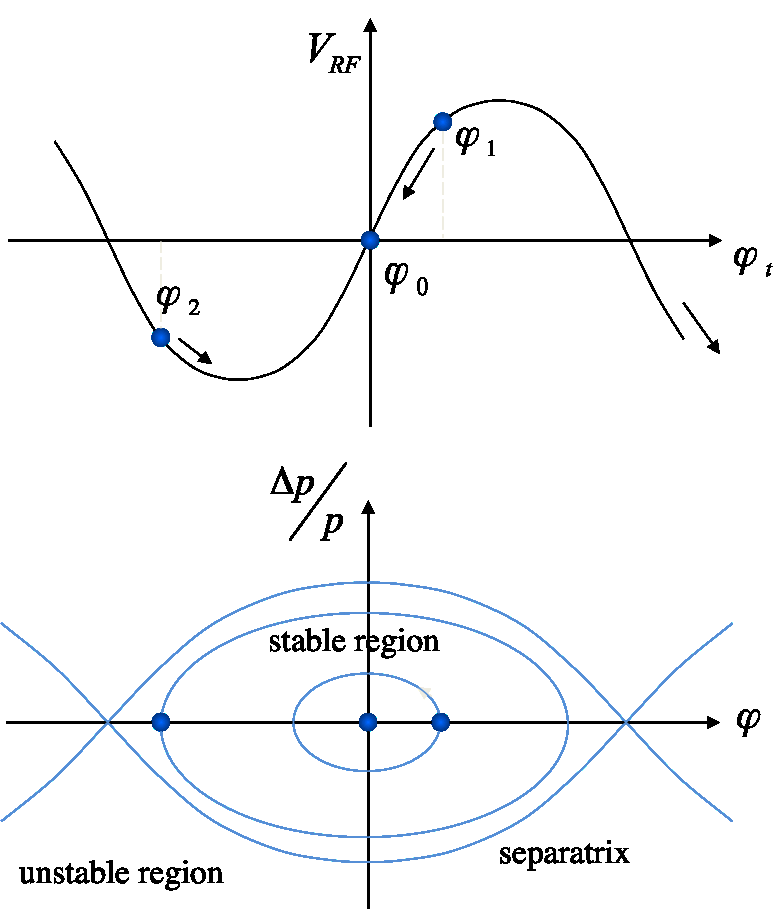
\includegraphics[height=.35\paperheight]{images/chapter1/psp_diagram}}
	\subbottom[Результаты моделирования с трансфер-матрицами третьего порядка\label{fig:PSP:3rd-order}]{%
		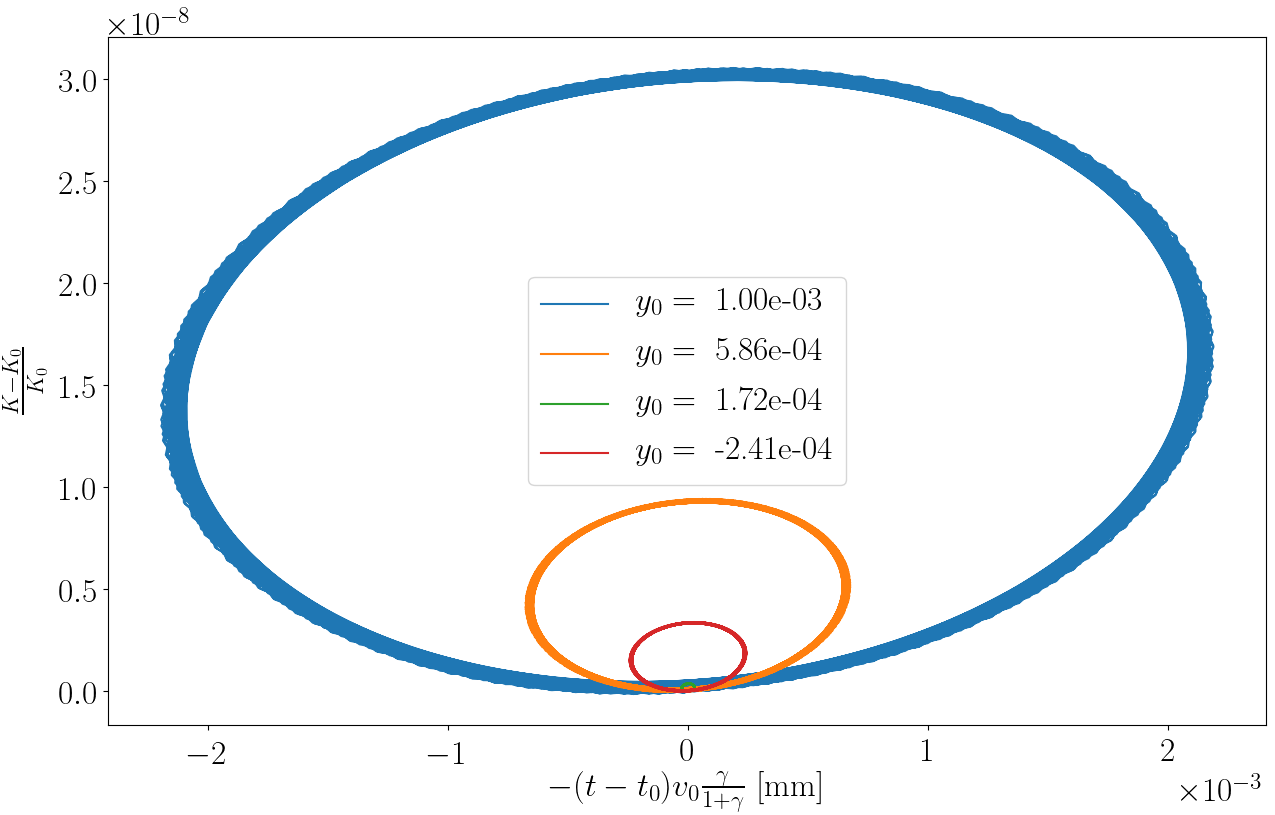
\includegraphics[height=.3\paperheight]{images/chapter1/psp_diagram_betatron}}
	\caption{Продольные фазовые портреты частиц в структуре с ВЧ продольной фокусировкой. Цветом различаются частицы с разными начальными сдвигами в вертикальной плоскости относительно референсной частицы; остальные координаты идентичны}
\end{figure}